% !TEX program = xelatex

%%%%%%%%%%%%%%%%%%%%%%%%%%%%%%%%%%%%%%%%%
% Thin Sectioned Essay
% LaTeX Template
% Version 1.0 (3/8/13)
%
% This template has been downloaded from:
% http://www.LaTeXTemplates.com
%
% Original Author:
% Nicolas Diaz (nsdiaz@uc.cl) with extensive modifications by:
% Vel (vel@latextemplates.com)
%
% License:
% CC BY-NC-SA 3.0 (http://creativecommons.org/licenses/by-nc-sa/3.0/)
%
%%%%%%%%%%%%%%%%%%%%%%%%%%%%%%%%%%%%%%%%%

%----------------------------------------------------------------------------------------
%	PACKAGES AND OTHER DOCUMENT CONFIGURATIONS
%----------------------------------------------------------------------------------------

\documentclass[a4paper, 11pt]{article} % Font size (can be 10pt, 11pt or 12pt) and paper size (remove a4paper for US letter paper)
\usepackage[table]{xcolor}
\usepackage{fontspec}
\definecolor{keycolor}{RGB}{172, 42, 42}
\definecolor{mbleu}{RGB}{64,96,127}
\definecolor{vimvert}{RGB}{46, 139, 87}
\usepackage{hyperref}

% \setmainfont{Avenir Next}
% \setsansfont{Avenir Next}

\usepackage{xeCJK}

\usepackage{geometry}
\geometry{left=2.54cm, top=2.54cm, right=2.54cm, bottom=2.54cm}
\usepackage{subcaption}
\usepackage{tikz}
\usetikzlibrary{tikzmark}
\usepackage{listings}
\usepackage{color}
\usepackage{forest}
\usepackage{float}
\usepackage{makecell}
\usepackage[binary-units]{siunitx}
\usepackage{subfigure} %插入多图时用子图显示的宏包

\lstset{
basicstyle=\small,%
escapeinside=``,%
keywordstyle=\color{blue} \bfseries,% \underbar,%
identifierstyle={},%
commentstyle=\color{blue},%
stringstyle=\ttfamily,%
%labelstyle=\tiny,%
extendedchars=false,%
linewidth=\textwidth,%
numbers=left,%
numberstyle=\tiny \color{blue},%
frame=trbl%
}
 
\newcounter{code}
\lstnewenvironment{code}[3][C++]%
  {%
    \renewcommand\lstlistingname{代码}
    \lstset{% frame=tb,
    language=#1,
    caption=#2,
    label=#3
    }
  }{}

% \usepackage{fancyhdr}
% \usepackage{lastpage}
% \pagestyle{fancy}
% \fancyhf{}
% \fancyfoot[R]{第 \thepage 页,共 \pageref{LastPage} 页}
% % \fancyfoot[C]{\thepage/\pageref{LastPage}}
% \renewcommand{\headrulewidth}{0pt} 
% \renewcommand{\footrulewidth}{0.4pt} 
\renewcommand{\lstlistingname}{Code} % Listing->Code

% \usepackage[protrusion=true,expansion=true]{microtype} % Better typography
\usepackage{graphicx} % Required for including pictures
\usepackage{wrapfig} % Allows in-line images
\usepackage{newfloat}
\usepackage{amsmath}
\usepackage{multirow}

\usepackage{mathpazo} % Use the Palatino font
\usepackage[T1]{fontenc} % Required for accented characters
\linespread{1.2} % Change line spacing here, Palatino benefits from a slight increase by default
% \setlength{\parskip}{0.2em}

\usepackage{indentfirst}
\setlength{\parindent}{2em}

\makeatletter
\renewcommand\@biblabel[1]{\textbf{#1.}} % Change the square brackets for each bibliography item from '[1]' to '1.'
\renewcommand{\@listI}{\itemsep=0pt} % Reduce the space between items in the itemize and enumerate environments and the bibliography

\renewcommand{\maketitle}{ % Customize the title - do not edit title and author name here, see the TITLE block below
\begin{center} % Right align
{\LARGE\@title} % Increase the font size of the title

\large{\@subtitle}

\vspace{1em} % Some vertical space between the title and author name

{\large\@author} % Author name
% \\\@date % Date

% \vspace{1.5em} % Some vertical space between the author block and abstract
\end{center}
}

\renewcommand{\figurename}{图}
\renewcommand{\tablename}{表}

%----------------------------------------------------------------------------------------
%	TITLE
%----------------------------------------------------------------------------------------

\title{\textbf{操作系统实验项目}\\ % Title
} % Subtitle
\newcommand\@subtitle{监控程序控制用户程序的执行}

\author{郑戈涵\quad 17338233\quad 931252924@qq.com} % Institution

\date{2020年5月3日} % Date


%----------------------------------------------------------------------------------------

\begin{document}

\maketitle % Print the title section

%----------------------------------------------------------------------------------------
%	ABSTRACT AND KEYWORDS
%----------------------------------------------------------------------------------------

\renewcommand{\abstractname}{摘要} % Uncomment to change the name of the abstract to something else

\begin{abstract}
  本次实验总共完成两个任务:获取计算机硬件系统的控制权和控制用户程序的执行
\end{abstract}

% \hspace*{3,6mm}\texttt{Keywords:} lorem , ipsum , dolor , sit amet , lectus % Keywords

\vspace{1em} % Some vertical space between the abstract and first section

\setcounter{tocdepth}{2}
\renewcommand{\contentsname}{目录}
\tableofcontents

% \vspace{2em} % Some vertical space between the abstract and first section

\pagebreak

\section{实验目的}

% 问题、方法、实验目的、意义
\begin{enumerate}
  \item 了解监控程序执行用户程序的主要工作
  \item 了解一种用户程序的格式与运行要求
  \item 加深对监控程序概念的理解
  \item 掌握加载用户程序方法
  \item 掌握几个BIOS调用和简单的磁盘空间管理
\end{enumerate}


\section{实验要求}

\begin{enumerate}
  \item 知道引导扇区程序实现用户程序加载的意义
  \item 掌握COM/BIN等一种可执行的用户程序格式与运行要求
  \item 将自己实验一的引导扇区程序修改为3-4个不同版本的COM格式程序,每个程序缩小显示区域,在屏幕特定区域显示,用以测试监控程序,在1.44MB软驱映像中存储这些程序。
  \item 重写1.44MB软驱引导程序,利用BIOS调用,实现一个能执行COM格式用户程序的监控程序。
  \item 设计一种简单命令,实现用命令交互执行在1.44MB软驱映像中存储几个用户程序。
  \item 编写实验报告,描述实验工作的过程和必要的细节,如截屏或录屏,以证实实验工作的真实性
\end{enumerate}

\section{实验内容}

% 输入、输出形式,使用的数据结构,算法的描述,算法正确性说明,算法分析,算法实现所需变量,没有代码
\subsection{获取计算机硬件系统的控制权}

\begin{enumerate}
  \item 将自己实验一的引导扇区程序修改为一个COM格式程序,程序缩小显示区域,在屏幕第一个1/4区域显示,显示一些信息后,程序会结束退出,可以在DOS中运行。在1.44MB软驱映像中制定一个或多个扇区,存储这个用户程序a。
  \item 将自己实验一的引导扇区程序修改为第二、第三、第四个的COM格式程序,程序缩小显示区域,在屏幕第二、第三、第四个1/4区域显示,在1.44MB软驱映像中制定一个或多个扇区,存储用户程序b、用户程序c、用户程序d。
\end{enumerate}

\subsection{控制用户程序的执行}

\begin{enumerate}
  \item 重写1.44MB软驱引导程序,利用BIOS调用,实现一个能执行COM格式用户程序的监控程序。程序可以按操作选择,执行一个或几个用户程序。解决加载用户程序和返回监控程序的问题,执行完一个用户程序后,可以执行下一个。
  \item 设计一种命令,可以在一个命令中指定某种顺序执行若干个用户程序。可以反复接受命令。
\end{enumerate}


\section{实验原理}
\subsection{BIOS调用}
BIOS是英文"Basic Input Output System"的缩略语,直译过来后中文名称就是"基本输入输出系统"。其实,它是一组固化到计算机内主板上一个ROM芯片上的程序,它保存着计算机最重要的基本输入输出的程序、系统设置信息、开机后自检程序和系统自启动程序。 其主要功能是为计算机提供最底层的、最直接的硬件设置和控制。

BIOS芯片中主要存放:

\begin{itemize}
  \item 自诊断程序:通过读取CMOSRAM中的内容识别硬件配置,并对其进行自检和初始化;
  \item CMOS设置程序:引导过程中,用特殊热键启动,进行设置后,存入CMOS RAM中;
  \item 系统自举装载程序:在自检成功后将磁盘相对0道0扇区上的引导程序装入内存,让其运行以装入DOS系统;
  \item 主要I/O设备的驱动程序和中断服务:由于BIOS直接和系统硬件资源打交道,因此总是针对某一类型的硬件系统,而各种硬件系统又各有不同,所以存在各种不同种类的BIOS,随着硬件技术的发展,同一种BIOS也先后出现了不同的版本,新版本的BIOS比起老版本来说,功能更强。
\end{itemize}

\subsection{BIOS中断例程}
BIOS中断服务程序是微机系统软、硬件之间的一个可编程接口,用于程序软件功能与微机硬件实现的衔接。DOS/Windows操作系统对软、硬盘、光驱与键盘、显示器等外围设备的管理即建立在系统BIOS的基础上。程序员也可以通过 对INT 5、INT 13等终端的访问直接调用BIOS终端例程。

常用的中断命令可以查看附录中的BIOS中断向量表(部分):\cite{wikiBIOS}

\section{实验过程}

这次实验的开放性也很强,为了方便以后的实验,虽然监控程序的功能可以在引导程序中直接实现,
我依然把他分开出来,作为一个简陋的内核程序。因此,这次实验需要5个步骤,分别是:

\begin{enumerate}
  \item 设计四个用户程序,内容与第一次实验类似
  \item 设计引导程序,将需要的扇区通过BIOS加载到内存中
  \item 设计监控程序,能够执行加载在内存中的程序
  \item 设计命令并对用户程序进行修改
  \item 生成镜像,在虚拟机中加载
\end{enumerate}
\subsection{用户程序设计}

为了理解bin和com的区别,我写了两个版本的代码。两个版本的用户程序的区别只有开头是否有org 100h,有的汇编生成后被认为是com文件,没有的被认为是bin。
除此之外,代码与第一次的基本一致,但是为了复用,我将一些重复出现的常量放在了头文件里,分别是Dn\_Rt,Up\_Rt,Up\_Lt,Dn\_Lt,delay,bigdelay,ddelay。

重复出现的变量在每个程序开头用宏的方式定义在上表中。 

% Please add the following required packages to your document preamble:
% \usepackage[table,xcdraw]{xcolor}
% If you use beamer only pass "xcolor=table" option, i.e. \documentclass[xcolor=table]{beamer}
\begin{table}[]
  \begin{tabular}{|l|l|}
    \hline
    \rowcolor[HTML]{FFFFFF} 
    {\color[HTML]{222222} \textbf{left}} & {\color[HTML]{222222} \textbf{字符运动的左边界}} \\ \hline
    top                                  & 字符运动的上边界                                 \\ \hline
    right                                & 字符运动的右边界                                 \\ \hline
    bottom                               & 字符运动的下边界                                 \\ \hline
    orix                                 & 字符运动的横坐标                                 \\ \hline
    oriy                                 & 字符运动的纵坐标                                 \\ \hline
  \end{tabular}
\end{table}

剩下的代码与第一次实验基本一致,只是修改了一些显示的特效,比如是否保留轨迹,显示的内容等。
以及字符运动的相关参数。四个程序的功能如下:
\begin{enumerate}
  \item LU.asm:每一次坐标变化颜色都会变化
  \item LD.asm:一个字符'H'在运动
  \item RU.asm:字符串"17338233OS"在运动
  \item RD.asm:字符碰到边界时变色
\end{enumerate}

\begin{figure}[H]
  \centering  %图片全局居中
  \subfigure[LU.img]{
    \label{Fig.sub.1}
    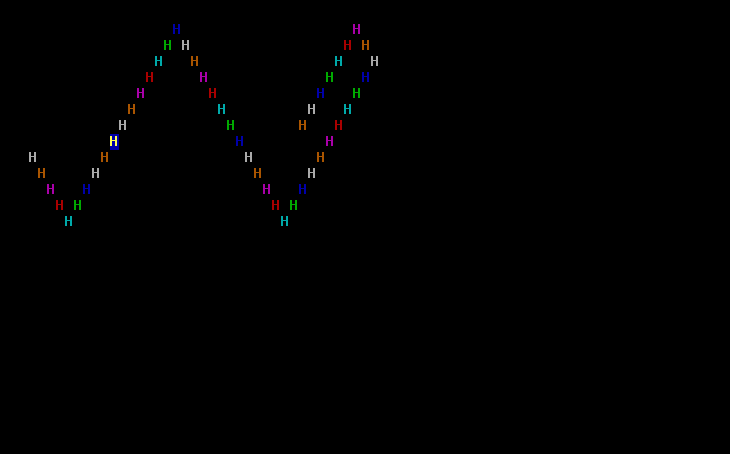
\includegraphics[width=0.45\textwidth]{LU.png}}
    \subfigure[RU.img]{
      \label{Fig.sub.2}
      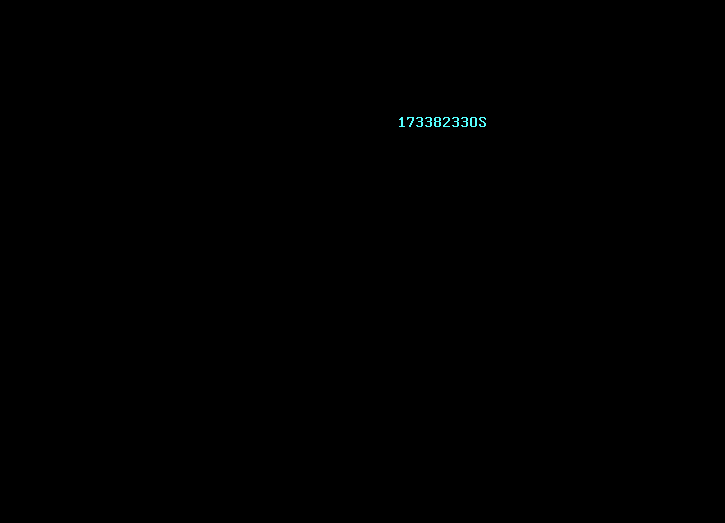
\includegraphics[width=0.45\textwidth]{RU.png}}
      \subfigure[LD.img]{
        \label{Fig.sub.3}
        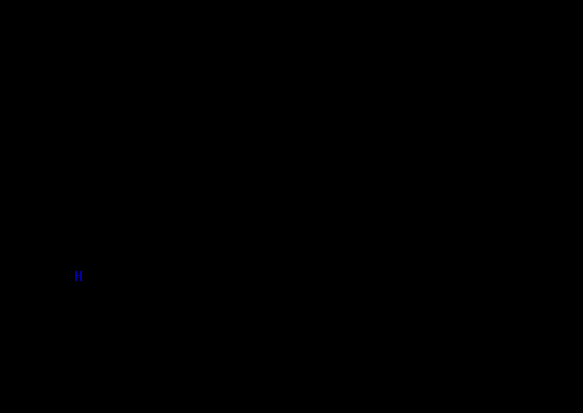
\includegraphics[width=0.45\textwidth]{LD.png}}
        \subfigure[RD.img]{
          \label{Fig.sub.4}
          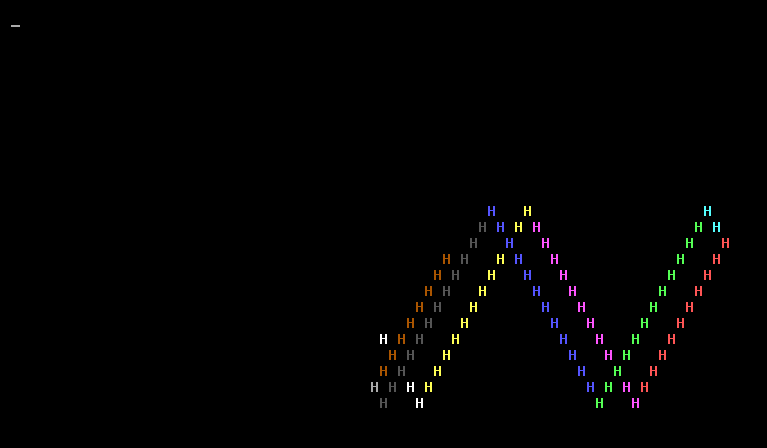
\includegraphics[width=0.45\textwidth]{RD.png}}
          \caption{用户程序的运行结果}
          \label{Fig.main}
        \end{figure}
        
由于部分程序中代码较多,超过了512字节,为方便计算盘块地址,
我将四个程序统一改成了1024个字节。写好代码后,将四个程序分别编译,并运行,运行结果如上图\ref{Fig.main}所示。

\subsection{引导程序设计}
引导程序的任务是将需要的盘块加载到内存中,然后跳转到监控程序。除此之外,为了让用户知道操作系统正在运行,还需要输出一些语句用于提示。

\subsubsection{提示字符串的输出}

由于之后的程序中输出需要反复使用,因此根据老师提供的代码,我将用系统调用的输出语句部分定义成宏放在了头文件里。
但是要注意的是,老师的代码是直接嵌入在代码中的,直接取出作为宏是不行的,必须在进入时保护现场,离开时恢复。
这样才能保证已有的数据不被破坏。这个宏在任何位置展开都不会有问题。
\paragraph{}
代码如下:
\begin{lstlisting}[language={[x86masm]Assembler},caption=字符串输出宏]
%macro PRINT 4
  pusha            ; 保护现场
  mov	ax, cs       ; 置其他段寄存器值与CS相同
  mov	ds, ax       ; 数据段
  mov	bp, %1       ; BP=当前串的偏移地址(%1)
  mov	ax, ds       ; ES:BP = 串地址
  mov	es, ax       ; 置ES=DS
  mov	cx, %2       ; CX = 串长(=%2)
  mov	ax, 1301h    ; AH = 13h(功能号)、AL = 01h(光标置于串尾)
  mov	bx, 0007h    ; 页号为0(BH = 0) 黑底白字(BL = 07h)
  mov dh, %3       ; 行号=%3
  mov	dl, %4       ; 列号=%4
  int	10h          ; BIOS的10h功能:显示一行字符
  popa             ; 恢复现场
%endmacro
\end{lstlisting}

输出字符串之后,由于读盘块的时间过短,用户几乎没办法看到显示的内容就被清屏了,因此我设置了一段延时,这段代码来自第一次实验。

\paragraph{}
代码如下:
\begin{lstlisting}[language={[x86masm]Assembler},caption=延时]
WaitLoop:
  dec word[count]			
  jnz WaitLoop				
  mov word[count],bigdelay
  dec word[dcount]			
  jnz WaitLoop
\end{lstlisting}

\subsubsection{监控程序和用户程序的加载}
加载程序需要用到BIOS的系统调用,可以使用int 13h来将软盘中的扇区加载到内存中。

\paragraph{}
代码如下:
\begin{lstlisting}[language={[x86masm]Assembler},caption=加载盘块到内存中]
LoadKernel:
  ;读软盘或硬盘上的若干物理扇区到内存的ES:BX处:
  mov ax,cs                ;段地址 ; 存放数据的内存基地址
  mov es,ax                ;设置段地址(不能直接mov es,段地址)
  mov bx, OffsetOfKernel  ;偏移地址; 存放数据的内存偏移地址
  mov ah,2                 ; 功能号
  mov al,1                 ;扇区数
  mov dl,0                 ;驱动器号 ; 软盘为0,硬盘和U盘为80H
  mov dh,0                 ;磁头号 ; 起始编号为0
  mov ch,0                 ;柱面号 ; 起始编号为0
  mov cl,2                 ;起始扇区号 ; 起始编号为1
  int 13H ;                调用读磁盘BIOS的13h功能
  ; 用户程序a.com已加载到指定内存区域中
\end{lstlisting}

为了方便修改,我将kernal.asm等文件的偏移量作为OffsetOfKernel等宏定义为在头文件。
加载其他盘块的代码基本相同,只是修改扇区号和扇区数(4个用户程序的扇区数为2)。
加载完成后,用jmp跳转到监控程序执行。

\subsection{监控程序设计}
首先设计镜像的结构,也就是确定各个盘块的位置,由于7c00h之前的位置不能使用,
因此选择之后的位置,并为各个盘块留足空间即可。我的安放位置如下:

\begin{lstlisting}[language={[x86masm]Assembler},caption=偏移量宏]
OffsetOfKernel equ  08100h
OffsetOfUserPrg1 equ  0A300h
OffsetOfUserPrg2 equ  0A700h
OffsetOfUserPrg3 equ  0AB00h
OffsetOfUserPrg4 equ  0AF00h
\end{lstlisting}


监控程序首先清屏,然后输出欢迎语句,清屏使用了BIOS的10号功能,为了能多次使用而不浪费空间,我将其定义成了子程序。
和print一样,需要保护现场和恢复现场。
\paragraph{}
代码如下:
\begin{lstlisting}[language={[x86masm]Assembler},caption=清屏]
  cls:         
  pusha
  mov ax, 0003h
  int 10h       ;清屏
  popa
  ret
\end{lstlisting}

而接下来两种文件格式便有较大的差别,首先要知道的com实际上和bin文件没有本质上的区别,
只是开头的org会影响整个文件的偏移量,比如org为100h,会使得整个文件中的label都出现100h的偏移,而不会影响ds,所以如果使用bin,
也就是自己决定偏移量,会少很多问题。而使用com时,需要注意数据段和代码段地址的计算。
\subsubsection{bin格式}
bin格式非常简单,因为宏对应的就是文件实际所在的物理地址,所以直接跳转不会出现其他问题,接下来通过BIOS的16号的01h调用获得键盘输入,
便可以按照用户的需求运行程序
代码如下:
\begin{lstlisting}[language={[x86masm]Assembler},label=WaitForKey,caption=获得键盘输入并跳转]
  WaitForKey:
	mov ah,0
	int 16h
	cmp al,'1'
	jz OffsetOfUserPrg1
	cmp al,'2'
	jz OffsetOfUserPrg2
	cmp al,'3'
	jz OffsetOfUserPrg3
	cmp al,'4'
	jz OffsetOfUserPrg4
  jmp WaitForKey
\end{lstlisting}

\subsubsection{com格式}
com格式由于用户程序并不知道自己的物理地址,需要修改段寄存器,包括cs和ds,而这一工作在bin格式的汇编里面也可以完成(没有意义),
所以监控程序需要完成段地址的计算和跳转,nasm汇编提供了\textit{call far}指令,可以完成段间转移,该指令完成的工作如下\cite{callfar}:

\begin{enumerate}
  \item push CS 
  \item push IP 
  \item jmp far ptr 标号
\end{enumerate}
所以接下来需要计算各个文件对应的段基址和偏移地址,由于org 100h,偏移地址ip是100h,而段基址通过文件所在物理地址通过以下公式计算得到
\begin{equation}
  ds=(OffsetOfUserPrg-100)/10
\end{equation}
理由是段地址左移4位加上偏移地址得到真正的物理地址,即
\begin{equation}
  PA(\text{physic address})= ds<<4 + offset
\end{equation}

按照镜像文件的设计,数据段的跳转地址如下:
\begin{lstlisting}[language={[x86masm]Assembler},label=WaitForKey,caption=用户程序对应的跳转地址]
	proc1 dw 100h,0xa00
	proc2 dw 100h,0xa20
	proc3 dw 100h,0xa60
	proc4 dw 100h,0xaa0
\end{lstlisting}

接下来完成代码,获得输入的部分和bin格式一样,而这次的跳转是去执行各自的段间转移
\begin{lstlisting}[language={[x86masm]Assembler},label=WaitForKey,caption=获得键盘输入并跳转]
  WaitForKey:
	mov ah,0
	int 16h
	cmp al,'1'
	jz program1
	cmp al,'2'
	jz program2
	cmp al,'3'
	jz program3
	cmp al,'4'
	jz program4
	jmp WaitForKey
\end{lstlisting}

段间转移代码如下:
\begin{lstlisting}[language={[x86masm]Assembler},label=WaitForKey,caption=获得键盘输入并跳转]
  program1:
  	call far [proc1]
	jmp start
  program2:
  	call far [proc2]
	jmp start
  program3:
  	call far [proc3]
	jmp start
  program4:
  	call far [proc4]
	jmp start
\end{lstlisting}
这样子便完成了监控程序的设计。


\subsection{用户程序的修改}

核心步骤已经完成,然而这样设计出来的操作系统,用户一旦进入了程序就无法离开。
无法按照用户的命令运行程序。因此,一种简单的设计是用户在运行程序时可以通过键盘输入恢复到选择的界面。
再选择想要运行的程序,修改内容如下:

\begin{enumerate}
  \item 在程序的开始时初始化各个变量
  \item 显示与程序相关的提示信息,以及离开程序的提示
  \item 获得用户的响应,并回到监控程序
\end{enumerate}

\subsubsection{程序开始时初始化变量}

按照上面的代码,如果在程序执行了一段时间后离开,内存中的数据会保留着被修改过的状态,若重新进入会从上次执行的位置开始,
按照我的理解,监控程序每次执行一个程序应该相当于从头开始执行,所以需要初始化。

\subsubsection{显示与程序相关的提示信息}

显示信息可以使用上面定义好的宏\textit{PRINT}。

\subsubsection{获取用户的响应}

在显示字符后获得响应需要用到BIOS的16号的01h调用,此调用与0h号调用不同,不阻塞程序的进行,
但是获得的是键盘的输入状态。因此用户可以在运行的同时输入。此时没有输入则回到循环开始,
有输入则通过0h号调用获得输入并比较跳转。我使用的比较的字符是Esc(27),各个字符对应的键盘扫描码可以在
\href{https://www.fountainware.com/EXPL/bios_key_codes.htm}{BIOS Key Codes}中找到。
这样用户在程序运行期间的任意时刻按下Esc键,都会回到监控程序的界面。
\paragraph{}
而两种格式返回监控程序的方法也是不同的,com版本中,由于我使用了\textit{call far}指令完成了段间转移,
从用户文件返回时需要使用\textit{retf}。bin版本的直接跳转返回即可。

此时如果重新将各个文件各种编译生成img,运行时会发现都是乱码,这是因为单独运行时是在主引导扇区7c00h,
而文件偏移量不正确,将其改成7c00h即可正常运行。

\subsection{镜像文件生成}
需要的代码已经写好,接下来将下述代码保存在run.sh,下面的是bin版本的
\begin{code}{生成镜像(bin):run.sh}{code:b-leaf-physical}
  #!/bin/bash
  outfile="os17338233.img"
  assembly=("myos1" "kernel" "LU" "LD" "RU" "RD")
  rm -f ${outfile}
  for asm_file in ${assembly[@]}
  do
    nasm ${asm_file}.asm -o ${asm_file}.bin
      cat ${asm_file}.bin >> "${outfile}"
      rm -f ${asm_file}.bin
      echo "[+] ${asm_file} done"
  done
  echo "[+] ${outfile} generated successfully."
\end{code}

下面是com版本的,使用了dd命令:
\begin{code}{生成镜像(com):run.sh}{code:b-leaf-physical}
  #!/bin/bash
  outfile="os17338233.img"
  assembly=("myos1" "kernel" "LU" "LD" "RU" "RD")
  rm -f ${outfile}
  for asm_file in ${assembly[@]}
  do
    nasm ${asm_file}.asm -o ${asm_file}.com
  done
  dd if=myos1.com of=${outfile} bs=512 count=1 2>/dev/null
  dd if=kernel.com of=${outfile} bs=512 seek=1 count=1 2>/dev/null
  dd if=LU.com of=${outfile} bs=512 seek=2 count=2 2>/dev/null
  dd if=LD.com of=${outfile} bs=512 seek=4 count=2 2>/dev/null
  dd if=RU.com of=${outfile} bs=512 seek=6 count=2 2>/dev/null
  dd if=RD.com of=${outfile} bs=512 seek=8 count=2 2>/dev/null
  for asm_file in ${assembly[@]}
  do
    rm -f ${asm_file}.com
      echo "[+] ${asm_file} done"
  done
  
  echo "[+] ${outfile} generated successfully."\end{code}
在命令行中执行即可生成镜像(.img)文件,在VMware中加载该镜像,查看结果。到此,实验结束。

\section{程序使用说明}
\subsection{实验环境}

\subsubsection{VMware Workstation 15}
VMware Workstation是VMware公司推出的一款桌面虚拟计算软件,具有Windows、Linux 版本。此软件可以提供虚拟机功能,使计算机可以同时运行多个不同操作系统。此次实验中用于运行镜像文件。
\subsubsection{nasm 2.13.02}
Netwide Assembler 是一款基于英特尔 x86 架构的汇编与反汇编工具。在此次实验中用生成二进制文件(.bin)
\subsubsection{wsl}
本次实验中用到了shell文件以批处理源代码生成镜像,整合于windows系统的wsl能够很方便的处理在windows系统上生成的文件。
\subsubsection{VSCode 1.44.2}
vscode能够方便的使用wsl和latex的pdf生成功能。加载虚拟机以外的所有任务都可以通过vscode完成。
% 如何编译和使用程序

\subsection{编译方法}

\subsubsection{系统要求}

生成镜像文件时,可以使用linux操作系统或者带wsl的windows系统。

\subsubsection{编译过程与参数}

在源代码目录下使用wsl,执行下列代码即可得到镜像文件os17338233.img。
\begin{code}{生成镜像}{code:b-leaf-physical}
  ./run.sh
\end{code}

\subsection{运行与演示}
两个版本的运行结果是一样的,下面以bin版本的为例
在虚拟机软件(此实验中为VMware Workstation)中创建虚拟机,将镜像作为软盘载入,设置随虚拟机启动后启动虚拟机即可。

运行结果如图 \ref{fig:run} 所示。

\begin{figure}[H]
  \centering
  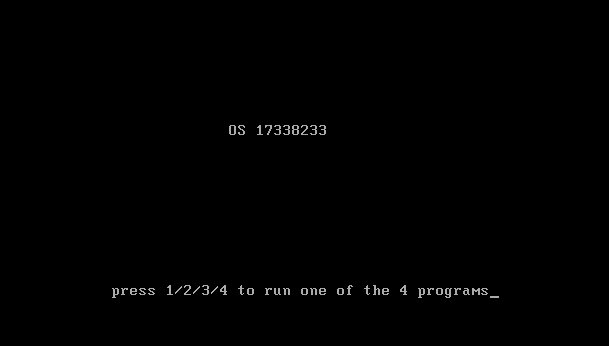
\includegraphics[width=0.8\linewidth]{run.png}
  \caption{运行过程截图}
  \label{fig:run}
\end{figure}
具体的演示过程可以查看已录制好的OSdemo.mkv
\section{总结与讨论}

% 特色、问题、教训、改进、收获


\subsection{特色,不足与改进}

本程序通过使用宏简化代码量,并使得常量易于变更,测试时更加方便。不足之处是用户程序比较简单,命令比较单调。
本实验我尝试着生成了两种不同格式的可执行文件,com版本由于计算段基址不能直接使用宏所以都为计算后手动填入,在测试时修改较为麻烦。修改程序时容易出现地址不一致的问题。
\subsection{收获}

通过本次实验,我复习了x86汇编,回顾了子程序的调用方式(call,入栈和出栈),了解了带参数的宏的使用以及头文件的包含,
宏\textit{PRINT}以及各个块的偏移量在代码中反复出现,非常实用。我也对操作系统的启动过程,还有BIOS的调用,
尤其是阻塞方式和非阻塞方式获取键盘输入有了一定的了解。
尝试编写两种格式的汇编时,我也对段间转移,物理地址的计算,汇编代码中标签的偏移量,org的意义有了更深入的理解。
同时,在本报告的编写过程中,我也练习了利用 \LaTeX 编写文档的能力。\cite{lamport94, cite}

\subsection{感想}
\paragraph{}
作为操作系统的第二个实验,代码量和第一次相比有较大的增加,并且完成的功能也更加复杂,为了理清项目的结构
我在实验开始时花了较长时间查询相关资料。
\paragraph{}
而实验过程中也遇到了不少问题,比如修改了字符串显示的位置有时候会导致看不到显示的内容,
或者使用的段寄存器不同(gs和es)也会导致输出乱码。前者后来并不能复现。后者是因为在不同文件里给段寄存器赋了不同的值导致数据偏移量错误,
说明段寄存器的功能要预先分配好,否则会出现冲突,这些问题刚出现时我完全不知道原因,复习了汇编之后才理解,说明写操作系统时,汇编能力是基础。
\paragraph{}
我遇到的最大的问题则是四个用户程序顺序的错乱,在完成bin版本的实验中,由于shell文件中我没有刻意安排各个镜像文件放置的位置,
运行时输入数字不仅并没有按照我的期望运行。虚拟机还发出了警报声并退出,从中我才明白了对bin格式来说物理位置的重要性,
将文件的物理地址与代码中的地址隔离开是非常有必要的,使用com格式就不会出现上述问题,只是运行的顺序有变化。
\paragraph{}
此外,这次实验由于子过程较多,我发现同样的调用结果,可以用非常多不同的指令,比如bin版本中\textit{kernel.asm}中跳转到其他段的部分,
如果把用户程序当成子过程,可以这样改:
\begin{lstlisting}[language={[x86masm]Assembler},caption=获得键盘输入并跳转]
  WaitForKey:
	mov ah,0
	int 16h
	cmp al,'1'
	jz program1
	cmp al,'2'
	jz program2
	cmp al,'3'
	jz program3
	cmp al,'4'
	jz program4
	jmp WaitForKey
  
  program1:
	call OffsetOfUserPrg1
	jmp start
  program2:
	call OffsetOfUserPrg2
	jmp start
  program3:
	call OffsetOfUserPrg3
	jmp start
  program4:
	call OffsetOfUserPrg4
	jmp start
  
\end{lstlisting}
经过测试,这样得到的结果和上面的一样,看似更加规整,但实际上和[\ref{WaitForKey}]完成了相同的工作,
却使用了更多的空间,在内存大小有限的情况下,还是更需要简洁有力的代码。因此我认为不必要使用call的场合,
用跳转指令是比较合适的。

\paragraph{}
这次遇到很多问题都花了不少时间才解决,因为我再使用bochs等调试工具时对命令不够熟悉,导致调试时并不能找到代码的问题,要希望在下次实验中我能够更高效的调试程序,比如使用bochs。
\begin{thebibliography}{99}
  
	\bibitem{lamport94}
  Leslie Lamport,
  \textit{\LaTeX: a document preparation system},
  Addison Wesley, Massachusetts,
  2nd edition,
  1994.
  \bibitem{cite}
  Contributors to Wikibooks,
  \textit{LaTeX Bibliography Management.}
  Wikibooks,
  2019., \\
  en.wikibooks.org/wiki/LaTeX/Bibliography\_Management.
  \bibitem{wikiBIOS}
  BIOS中断调用
  \textit{Wikipedia, The Free Encyclopedia}
  2019., \\
  https://zh.wikipedia.org/wiki/BIOS%E4%B8%AD%E6%96%B7%E5%91%BC%E5%8F%AB
  
  \bibitem{callfar}
  汇编语言入门:CALL和RET指令(一)
  鸾林居士,
  2018., \\
  https://blog.csdn.net/abc_12366/article/details/79774530  

\end{thebibliography}

\clearpage

\section{附录:BIOS中断向量表}
% Please add the following required packages to your document preamble:
% \usepackage[table,xcdraw]{xcolor}
% If you use beamer only pass "xcolor=table" option, i.e. \documentclass[xcolor=table]{beamer}
\makeatletter\def\@captype{table}\makeatother
  \caption{BIOS 中断向量表}
  \label{tab:BIOS_interrupt_table}
  \begin{tabular}{|
  >{\columncolor[HTML]{FFFFFF}}l |
  >{\columncolor[HTML]{FFFFFF}}l |}
  \hline
  {\color[HTML]{222222} \textbf{中断}} & {\color[HTML]{222222} \textbf{描述}}                                                                                                                                                                                                                                                                                                                                                \\ \hline
  {\color[HTML]{0B0080} INT 10h}     & {\color[HTML]{222222} \begin{tabular}[c]{@{}l@{}}显示服务 - 由BIOS或操作系统设定以供软件调用。\\ AH=00h  设定显示模式\\ AH=01h  设定游标形态\\ AH=02h  设置光标位置\\ AH=03h  获取光标位置与形态\\ AH=04h  获取光标位置\\ AH=05h  设置显示页\\ AH=06h  清除或滚动栏画面(上)\\ AH=07h  清除或滚动栏画面(下)\\ AH=08h  读取游标处字符与属性\\ AH=09h  更改游标处字符与属性\\ AH=0Ah  更改游标处字符\\ AH=0Bh  设定边界颜色\\ AH=0Eh  在TTY模式下写字符\\ AH=0Fh  获取当前显示模式\\ AH=13h  写字符串\end{tabular}} \\ \hline
  {\color[HTML]{222222} INT 11h}     & {\color[HTML]{222222} 返回设备列表。}                                                                                                                                                                                                                                                                                                                                                    \\ \hline
  {\color[HTML]{222222} INT 12h}     & {\color[HTML]{222222} 获取常规内存容量。}                                                                                                                                                                                                                                                                                                                                                  \\ \hline
  {\color[HTML]{A55858} INT 13h}     & {\color[HTML]{222222} \begin{tabular}[c]{@{}l@{}}低端磁盘服务。\\ AH=00h  复位磁盘驱动器。\\ AH=01h  检查磁盘驱动器状态。\\ AH=02h  读扇区。\\ AH=03h  写扇区。\\ AH=04h  校验扇区。\\ AH=05h  格式化磁道。\\ AH=08h  获取驱动器参数。\\ AH=09h  初始化硬盘驱动器参数。\\ AH=0Ch  寻道。 \end{tabular}}                                                                                  \\ \hline
  {\color[HTML]{222222} INT 16h}     & {\color[HTML]{222222} \begin{tabular}[c]{@{}l@{}}键盘通信例程。\\ AH=00h  读字符。\\ AH=01h  读输入状态。\\ AH=02h  读 Shift 键(修改键)状态。\\ AH=10h  读字符(增强版)。\\ AH=11h  读输入状态(增强版)。\\ AH=12h  读 Shift 键(修改键)状态(增强版)。\end{tabular}}                                                                                                                                                                     \\ \hline
  {\color[HTML]{222222} INT 19h}     & {\color[HTML]{0B0080} 加电自检之后加载操作系统。}                                                                                                                                                                                                                                                                                                                                              \\ \hline
  \end{tabular}

%----------------------------------------------------------------------------------------

\end{document}